%---------- COURSE INFORMATION ------------------------
\newcommand{\course}{CIS 444-01}
\newcommand{\coursetitle}{ADVANCED IT INFRASTRUCTURE}
\newcommand{\courseloc}{Raburn 210}
\newcommand{\coursetime}{Monday/Wednesday 1:30 p.m. - 2:45 a.m.}
\newcommand{\coursedesc}{Explore advanced concepts for the design and implementation of robust IT infrastructures. Understand infrastructure and design using expert command line interfaces to harden systems, secure access, configure file storage services, as well as other advanced topics in design and configuration of IT services.}
\newcommand{\coursesec}{01}
\newcommand{\coursecredithours}{3}
\newcommand{\courseprereq}{CIS 344.}
\newcommand{\coursedelmethod}{Traditional Classroom}

\newcommand{\courseobjectives}{
	\item Explain all aspects of IT infrastructure including: wiring, routing, servers, workstations, etc. [CIS Program Goal 1,2,4,5][COB Goals 2,3]
	\item Install and configure the following infrastructure components [CIS Program Goal 5,7,8,9][COB Goal 3]:
	\begin{enumerate}
		\item Routers and firewalls
		\item SMTP services
		\item DNS clients and servers
		\item Virtual Machines
		\item NFS
		\item SSH
		\item Kerberos, LDAP
		\item SNMP
	\end{enumerate}
}

\newcommand{\coursetopics}{
	\item System administration
	\item Virtual machines and hypervisors
	\item Performance tuning and optimization
	\item Infrastructure server software and configuration
	\item System and network auditing
	\item System and network hardening
}
\newcommand{\coursegrades}{
	Subject exams (2 exams @ 20\% each)\dotfillsmall 40\% \\
	Project work\dotfillsmall 30\% \\
	Final project\dotfillsmall 30\%
}
\newcommand{\coursetext}{
	\adjustbox{valign=c}{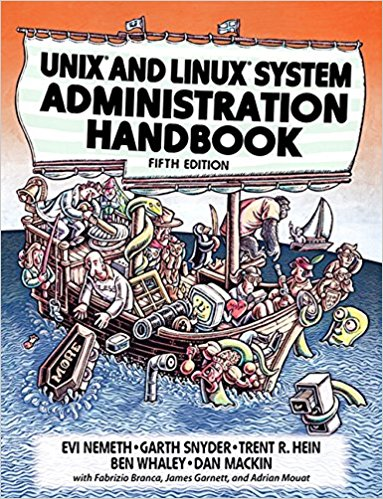
\includegraphics[width=1in]{img/cis-444}} & \hangindent .4in \textbf{Textbook:} Nemeth, E., Snyder, G., Hein, T., Whaley, B., Mackin, D. (2017). UNIX and Linux System Administration Handbook (5th Edition). Addison-Wesley Professional. ISBN-10: 0134277554 $\bullet$ ISBN-13: 978-0134277554.
}